\documentclass[a4paper,USenglish,cleveref,autoref,thm-restate,anonymous]{lipics-v2021}
%This is a template for producing LIPIcs articles. 
%See lipics-manual.pdf for further information.
%for A4 paper format use option "a4paper", for US-letter use option "letterpaper"
%for british hyphenation rules use option "UKenglish", for american hyphenation rules use option "USenglish"
%for section-numbered lemmas etc., use "numberwithinsect"
%for enabling cleveref support, use "cleveref"
%for enabling autoref support, use "autoref"
%for anonymousing the authors (e.g. for double-blind review), add "anonymous"
%for enabling thm-restate support, use "thm-restate"

%\graphicspath{{./graphics/}}%helpful if your graphic files are in another directory

\hideLIPIcs 

\ccsdesc{%
Theory of computation $\rightarrow$ 
Design and analysis of algorithms $\rightarrow$ 
Parameterized complexity and exact algorithms $\rightarrow$ 
Fixed parameter tractability}


% TODO 




\bibliographystyle{plainurl}
\newcommand{\citet}[1]{\cite{#1}}
\usepackage{graphicx}
\urlstyle{rm}
\def\UrlFont{\rm}
\usepackage{graphicx} 
\newif\iflong
\newif\ifshort

% comment the below line out for short version
\longtrue

\iflong
\else
\shorttrue
\fi
\usepackage{tikz}
\usepackage{booktabs}

\keywords{parameterized complexity, NLC-width, rank-width, decision trees, partially defined Boolean formulas}

\usepackage[noend]{algpseudocode}
\usepackage{algorithm,algorithmicx}
\newcommand{\NULL}{\textnormal{\texttt{nil}}}

\algnewcommand\algorithmicinput{\textbf{Input:}}
\algnewcommand\INPUT{\item[\algorithmicinput]}

\algnewcommand\algorithmicoutput{\textbf{Output:}}
\algnewcommand\OUTPUT{\item[\algorithmicoutput]}

% decision trees and parameters
\newcommand{\DTL}{\probfont{DTS}}
\newcommand{\DTLh}{\probfont{DTD}}
\newcommand{\MSS}{\textup{MSS}}
\newcommand{\MNE}{\min_{\#}}
\newcommand{\GIL}{G^+_I}


\newcommand{\inst}{I}
\newcommand{\MIHS}{\probfont{MIHS}}

% \newcommand{\HD}{\delta}
% \newcommand{\MHD}{\delta_{\max}}
% \newcommand{\DMAX}{D_{\max}}

% \newcommand{\GD}{D}
% \newcommand{\IV}{I}

\usepackage{todonotes}
\presetkeys%
    {todonotes}%
    {inline,backgroundcolor=yellow}{}

%table stuff?
\usepackage{booktabs}
\usepackage{multirow}
%\usepackage{floatrow}

\usepackage{amsthm,amsmath,amssymb}
\usepackage{enumerate,verbatim}
\usepackage{xspace}

\usepackage{tikz,tikz-cd}
\usetikzlibrary{arrows,cd,positioning,shapes,patterns}


\usepackage[draft,author=]{fixme}
\fxsetup{theme=color}
%\newcommand{\todo}[1]{\fxerror{#1}}
\newcommand{\warn}[1]{\fxwarning{#1}}
\renewcommand{\note}[1]{\fxnote{#1}}
\newcommand{\nb}[1]{\todo{\scriptsize #1}}



\newcommand{\SB}{\{\,}
\newcommand{\SM}{\;{|}\;}
\newcommand{\SE}{\,\}}
\newcommand{\PP}{\mathcal{P}}
\newcommand{\QQ}{\mathcal{Q}}
\newcommand{\III}{\mathcal{I}}
\newcommand{\SSS}{\mathcal{S}}
\newcommand{\RRR}{\mathcal{R}}
\newcommand{\DDD}{\mathcal{D}}
\newcommand{\FFF}{\mathcal{F}}
\newcommand{\TTT}{\mathcal{T}}
\newcommand{\VVV}{\mathcal{V}}
\newcommand{\XXX}{\mathcal{X}}

\newcommand{\RR}{\mathcal{R}} 

\newcommand{\Z}{\mathbb{Z}}
\newcommand{\Nat}{\mathbb{N}}
\newcommand{\downcl}[2]{D_{#1}(#2)}
\newcommand{\pref}{P_{\leq^V}}
\newcommand{\suff}{S_{\leq^V}}

\newcommand{\bigoh}{\mathcal{O}}
\newcommand{\littleoh}{o}

 
 


\newcommand{\cc}[1]{{\mbox{\textnormal{\textsf{#1}}}}\xspace}  %% Complexity class
\newcommand{\cocc}[1]{{\mbox{\textrm{co}\textnormal{\textsf{#1}}}}\xspace}  %% Complexity class

\newcommand{\integers}{\mathbb{Z}}
\renewcommand{\P}{\cc{P}}
\newcommand{\NP}{\cc{NP}}
\newcommand{\coNP}{\cc{co-NP}}
\newcommand{\FPT}{\cc{FPT}}
\newcommand{\XP}{\cc{XP}}
\newcommand{\Weft}{{\cc{W}}}
\newcommand{\W}[1]{{\Weft}{{\textnormal[#1\textnormal]}}}
\newcommand{\paraNP}{\cc{paraNP}}
\newcommand{\paraNPs}{\cc{pNP}}


\newcommand{\fpt}{fixed-pa\-ra\-me\-ter trac\-ta\-ble\xspace}

\newcommand{\tuple}[1]{\langle{#1}\rangle}  % Tuple
\newcommand{\pn}[1]{\textsc{#1}}
\newcommand{\hy}{\hbox{-}\nobreak\hskip0pt}

%\newcommand{\citet}[1]{\citeauthor{#1}~\shortcite{#1}\xspace}
\newcommand{\nn}{\mathbb{N}}

\newcommand{\bigO}[1]{\ensuremath{{\mathcal O}(#1)}}
\newcommand{\bigOstar}[1]{\ensuremath{{\mathcal O}^*(#1)}}

\newcommand{\probfont}[1]{\textnormal{\textsc{#1}}}

%\newcommand{\stw}{dependency treewidth}



%\newcommand{\RAPROG}{\probfont{Proportionality Graph Allocation}}
\newcommand{\RAENVG}{\probfont{(Locally) Envy-Free Allocation}}
\newcommand{\RAENVGNL}{\probfont{Envy-Free Allocation}}
\newcommand{\RAENVGL}{\probfont{Locally Envy-Free Allocation}}

\newcommand{\EFA}{\textsc{EFA}}
\newcommand{\LEFA}{\textsc{LEFA}}

\newcommand{\FCGENVPROP}{envy-free}
\newcommand{\FCGENV}{locally envy-free}
\newcommand{\FCGPROP}{proportional}

\newcommand{\AT}{T_A}
\newcommand{\RT}{T_R}
\newcommand{\mundef}{\textup{undef}}
\newcommand{\BS}{\textup{BS}}

\newcommand{\RofRT}{R}
\newcommand{\RTBUN}{\textup{BUN}}
\newcommand{\RTVEC}{\vec{b}}
\newcommand{\RTVECSET}{\mathcal{B}}

\newcommand{\rall}{\alpha}
\newcommand{\itf}{\vec{u}}
\newcommand{\new}[1]{}
\newcommand{\valn}{\beta}
\newcommand{\VR}{\RRR}


\newcommand{\prop}[1]{#1}
\newcommand{\noprop}[1]{}
\newcommand{\bunmin}{\alpha_{\min}}
\newcommand{\bunmax}{\alpha_{\max}}
\newcommand{\propmax}{\beta}
\usepackage{boxedminipage}

\newcommand{\MCC}{\probfont{Multicolored Clique}}

\newcommand{\pbDef}[3]{%
\noindent
\begin{center}
\begin{boxedminipage}{0.98 \columnwidth}
#1\\[5pt]
\begin{tabular}{l p{0.70 \columnwidth}}
Input: & #2\\
Question: & #3
\end{tabular}
\end{boxedminipage}
\end{center}
}

\newcommand{\pbDefP}[4]{%
\noindent
\begin{center}
\begin{boxedminipage}{0.98 \columnwidth}
#1\\[5pt]
\begin{tabular}{l p{0.70 \columnwidth}}
Input: & #2\\
Parameter: & #3\\
Question: & #4
\end{tabular}
\end{boxedminipage}
\end{center}
}


\newcommand{\lc}{l}
\newcommand{\rc}{r}

\newcommand{\reaches}{r}


\newcommand{\CCC}{\mathcal{C}}

\newcommand{\ol}[1]{\overline{#1}}
\newcommand{\Card}[1]{|#1|}
\let\phi=\varphi
\let\epsilon=\varepsilon 
\def\hy{\hbox{-}\nobreak\hskip0pt} 
% Name for our encoding and for the whole approach
\newcommand{\enc}{DT\_pb}
\newcommand{\ench}{DT\_hyb}
\newcommand{\slv}{DT\_rec}
% Subsampling strategies
\newcommand{\stratrand}{RandSelect}
\newcommand{\stratlearn}{TreeSelect}
\newcommand{\stratleaf}{LeafSelect}
\newcommand{\stratinc}{MonotonicSelect}
% Feature reduction
\newcommand{\redcon}{\text{FR}}
\newcommand{\redgreedy}	{$\redcon_{\text{greedy}}$}
\newcommand{\redmaxsat}	{$\redcon_{\text{maxsat}}$}
\newcommand{\redrand}	{$\redcon_{\text{rand}}$}
\newcommand{\reddec}	{$\redcon_{\text{back}}$}

% reduction flags
\newcommand{\redinit}{RI}
\newcommand{\redinc}{RC}

\newcommand{\dif}{\text{\specialfont{diff}}}
\newcommand{\dom}{\text{\specialfont{dom}}}
\newcommand{\siz}{\text{\specialfont{size}}}
\newcommand{\solsize}{\text{\specialfont{sol}}}

\newcommand{\parameter}[1]{\text{\normalfont{\sffamily #1}}}
 

\newcommand{\var}{\text{\specialfont{feat}}}
\newcommand{\feat}{\text{\specialfont{feat}}}
\newcommand{\thres}{\lambda}

\newcommand{\leaf}{\text{\specialfont{leaf}}}



\newcommand{\specialfont}[1]{{\normalfont\slshape #1}}

\newcommand{\rtw}{\text{\specialfont{rtw}}}
\newcommand{\tw}{\text{\specialfont{tw}}}
\newcommand{\cw}{\text{\specialfont{cw}}}
\newcommand{\rw}{\text{\specialfont{rw}}}
\newcommand{\dep}{\text{\specialfont{dep}}}
\newcommand{\ghtw}{\text{\specialfont{ghtw}}}
\newcommand{\htw}{\text{\specialfont{htw}}}




\begin{document}
%\raggedright\pagestyle{empty}\nolinenumbers

\ifshort
\title{Fixed-Parameter Tractability of\\  Learning Small Decision Trees}
\fi
\iflong
\title{Fixed-Parameter Tractability of\\  Learning Small Decision Trees\\(full paper)}
\fi

\author{TODO}{~}{~}{}{}
\authorrunning{~}
\titlerunning{}
\maketitle


\begin{abstract}
We consider the NP-hard problem of finding a smallest decision tree which represents a given partially defined Boolean formula. We establish fixed-parameter tractability of the problem with respect to the NLC-width of the instance. We formulate a dynamic programming procedure which utilizes the NLC-decomposition of the instance. For this to work, we establish a succinct representation of partial solutions, so that the space and time requirements of each dynamic programming step remain bounded in terms of the NLC-width.
\end{abstract}
 
\newpage
\clearpage
\setcounter{page}{1}

\section{Introduction}
Decision trees have proved to be extremely useful tools for the describing, classifying, generalizing data~\cite{Larose05,Murthy98,Quinlan86}. In this paper, we consider decision trees for {\it classification instances (CIs)}, consisting of a finite set $E$ of {\it examples} (also called {\it feature vectors}) over a finite set $F$ of {\it features}. Each example $e\in E$ is a function $e:F\rightarrow \{0,1\}$ which determines whether the feature~$f$ is true or false for $e$.  Moreover, $E$ is given as a partition $E^+ \uplus E^-$ into positive and negative examples. For instance,  examples could represent medical patients and features diagnostic tests; a patient is positive or negative corresponding to whether they have been diagnosed with a certain disease or not. CIs are also called {\it partially} or {\it incompletely defined Boolean functions}, as we can consider the features as Boolean variables, and examples as  truth assignments that evaluate to 0 (for positive examples) or 1 (for negative examples). CIs have been studied as a key concept for the logical analysis of data and in switching theory \cite{BorosCHIKM11,Boros03,BorosGHIK95,BorosIbarakiMakino03,   CramaHammerIbaraki88,IbarakiCramaHammer11,Mccluskey65}.

Because of their simplicity, decision trees are particularly attractive for providing interpretable models of the underlying CI, an aspect whose importance has been strongly emphasized over the recent years~\cite{DarwicheHirth20,DoshivelezKim17,GoodmanFlaxman17,Lipton18,Monroe18}. In this context, one prefers {\it small trees}, as they are easier to interpret and require fewer tests to make a classification. Small trees are also preferred in view of the parsimony principle (Occam’s Razor) since small trees are expected to generalize better to new data~\cite{Bessiere09}. However, finding a small decision tree, as formulated in the following decision problem, is NP-complete~\cite{HyafilRivest76}. 

\begin{quote}
\probfont{Minimum Decision Tree Size (\DTL):} given a CI $E=E^+ \uplus E^-$ and an integer $s$, is there a decision tree with at most $s$ nodes for $E$?
\end{quote}

Given this complexity barrier, we propose a fixed-parameter algorithm for the problem, which exploits the input CI's hidden structure. The {\it incidence graph} of a CI is the bipartite graph $G_I(E)$ whose vertices are the examples on one side and the features on the other, where an example $e$ is adjacent with a feature $f$ if and only if $e(f)=1$. Figure~\ref{fig:example} shows a CI and a smallest decision tree for it, as well as the incidence graph.

\begin{figure}[b]
\small
\begin{minipage}{0.33\linewidth}
\centering
\begin{tabular}{@{}c@{~~}c@{~~}c@{~~}c@{~~}c@{}}
$E$  & $f_1$ & $f_2$ & $f_3$ & $f_4$ \\
\midrule
$e_1 \in E^-$ & 0 & 0 &1 & 0   \\
$e_2 \in E^-$ & 0 & 0 &1 & 1   \\
$e_3\in E^-$ & 0 & 1 &1 & 0 \\
$e_4\in E^-$ & 1 & 1 & 0 & 0   \\
$e_5\in E^+$ & 1 & 0 & 0 & 1  \\
$e_6\in E^+$ & 1 & 0 & 1 & 1  \\
\end{tabular}
\end{minipage}%
\begin{minipage}{0.33\linewidth}
\centering
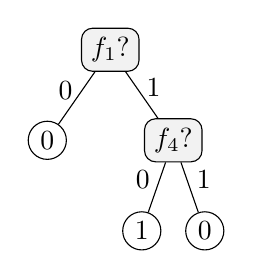
\begin{tikzpicture}[xscale=0.8,yscale=1.15]
\tikzstyle{test} = [draw, rectangle, rounded corners, fill=gray!10]
\tikzstyle{p} = [draw, circle, rounded corners, inner sep=2pt]
\tikzstyle{n} = [draw, circle, rounded corners, inner sep=2pt]
\draw  (0,0) node [test] (A) {$f_1$?}
(1,-1) node [test] (C) {$f_4$?}
(-1,-1) node [n] (B) {0}
(1.5,-2)  node [n] (E) {0}
(0.5,-2)  node [p] (D) {1};
\draw (A) -- (B) node [left,pos=0.35] {0};
\draw (A) -- (C) node [right,pos=0.35] {1};
\draw (C) -- (D) node [left,pos=0.35] {0};
\draw (C) -- (E) node [right,pos=0.35] {1};
\end{tikzpicture}
\end{minipage}%
\begin{minipage}{0.33\linewidth}
\centering
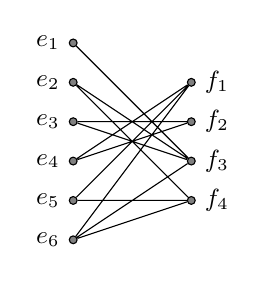
\begin{tikzpicture}[xscale=1.5,yscale=0.5]
\small
\tikzstyle{node} = [draw, circle, rounded corners, fill= gray, inner sep=1pt]
\draw
(0,0) node [node,label=left:$e_1$] (e1) {}
(0,-1) node [node,label=left:$e_2$] (e2) {}
(0,-2) node [node,label=left:$e_3$] (e3) {}
(0,-3) node [node,label=left:$e_4$] (e4) {}
(0,-4) node [node,label=left:$e_5$] (e5) {}
(0,-5) node [node,label=left:$e_6$] (e6) {}
(1,-1) node [node,label=right:$f_1$] (f1) {}
(1,-2) node [node,label=right:$f_2$] (f2) {}
(1,-3) node [node,label=right:$f_3$] (f3) {}
(1,-4) node [node,label=right:$f_4$] (f4) {}
(e1)--(f3) (e2)--(f3) (e2)--(f4) (e3)--(f2) (e3)--(f3) (e4)--(f1) (e4)--(f2) (e5)--(f1) (e5)--(f4) (e6)--(f1) (e6)--(f3) (e6)--(f4);
\end{tikzpicture}
\end{minipage}%
\caption{A CI $E=E^+\uplus E^-$ with six examples and four features (left), a decision tree with~5 nodes that classifies $E$ (middle), the incidence graph $G_I(E)$ (right).} \label{fig:example}
\end{figure}

Key to our algorithm are new notions for succinctly representing decision trees that correspond to subtrees of the incidence graph's tree decomposition.  Based on that, we can carry out a dynamic programming (DP) procedure along the tree decomposition.  

While the DP approach using treewidth is quite well understood and can often be quite easily designed for problems on graphs (or more generally problems whose solutions can be represented in terms of the graph for which the tree decomposition is given), the same DP approach can become rather involved if applied to problems whose solutions have
no or only minor resemblence to the graph for which one is given a tree decomposition. Probably the most prominent example for this is the celebrated result by Bodlaender~\cite{Bodlaender96}, where he uses a DP approach on an approximate tree decomposition to compute the exact treewidth of a graph; here, the solutions are tree decompositions, which are complex structures that cannot easily be represented in terms of the graph. Other prominent examples include a DP approach to compute the exact treedepth~\cite{DBLP:conf/icalp/ReidlRVS14} or clique-width~\cite{DBLP:journals/jgaa/EspelageGW03} using an optimal tree decomposition.  We face a similar problem, since solutions in our case are decision trees that do not bear any resemblence to the incidence graph for which we are given the tree decomposition. The main obstacle to overcome, therefore, is the design of the DP-records for our DP algorithm. That is, a record for a node $b$ in a tree decomposition for the incidence graph of $E$ needs to provide a compact representation of partial solutions, i.e. partial solutions in the sense that they represent the part of the solution for the whole instance $E$ that corresponds to the sub-instance induced by all features and examples contained in the bags in the subtree of the tree
decomposition rooted at the current node $b$. We overcome this obstacle in Section~\ref{sec:twfpt}, where we also provide intuitive descriptions and motivation for the definition of the records (Subsection~\ref{ssec:mainideas}).

\ifshort
{\it The full proof of statements marked with $(\star)$ can be found  in the full version of this paper.}
\fi

\section{Preliminaries}\label{chap:prelims}

\subsection{Parameterized Complexity}
We give some basic definitions of Parameterized Complexity and refer for a more in-depth treatment to other sources \cite{CyganFKLMPPS15,DowneyFellows13}. Parameterized complexity considers problems in a two-dimensional
setting, where a problem instance is a pair $(I,k)$, where $I$ is the main part and~$k$ is the parameter. A parameterized problem is {\it fixed-parameter tractable} if there exists a computable function $f$ such that instances $(I,k)$ can be solved in time $f(k) \|I\|^{O(1)}$.

\subsection{Graphs and NLC-width}

We will assume that the reader is familiar with basic graph theory (see, e.g. \cite{Diestel00,BangjensenGutin09}).  We
consider (vertex and edge labelled) undirected graphs. Let $G=(V,E)$ be an undirected graph. We write $V(G)=V$ and $E(G)=E$ for the sets of vertices and edges of $G$, respectively. We denote an edge between $u \in V$ and $v \in V$ as $\{u,v\}$. For a set $V' \subseteq V$ of vertices we let $G[V']$ denote the graph induced by the vertices in $V'$, i.e. $G[V']$ has vertex set $V'$ and edge set $E \cap \SB \{u,v\} \SM u,v \in V' \SE$ and we let $G - V'$ denote the graph $G[V \setminus V']$. For a set $E' \subseteq E$ of edges we let denote $G-E'$ the graph with vertex set $V$ and edge set $E\setminus E'$. 

Node label control-width (NLC-width) is a graph parameter, defined as follows~\cite{Wanke94}: Let $k \in \mathbb{N}$ be a positive integer. A $k$-NLC-expression consists of a rooted subcubic tree such that:

\begin{enumerate}
\item Every leaf is labelled with a label $i \in [k]$; this corresponds to a graph with a single vertex which has a label~$i$.
\item Every non-leaf node with one child is labelled with a function $R:[k] \to [k]$. This corresponds to taking the labelled graph corresponding to the child and for every $i \in \{1,\ldots,k\}$, if a vertex has label~$i$, changing this label to be $R(i)$ instead.
\item Every non-leaf node with two children is labelled with a $k \times k$ $\{0,1\}$ matrix~$M$. This corresponds to taking the disjoint union of the graphs corresponding to its children~$G_1$ and~$G_2$, and then for $i,j \in [k]$, adding an edge from all vertices lablled~$i$ in~$G_1$ to all vertices labelled~$j$ in~$G_2$ if and only if $M_{i,j}=1$.
\item The root node corresponds to the resulting labelled graph.
\end{enumerate}

The NLC-width~$NLC(G)$ of a graph~$G$ is the minimum~$k$ for which~$G$ has a $k$-NLC-expression.
A $k$-NLC-expression is {\it nice} if every relabelling node has a function $R:[k] \to [k]$ such that for some $i,j \in [k]$, $R(i)=j$ and $R(\ell)=\ell$ for all $\ell \in [k] \setminus \{i\}$.
%KD: Proably want to prove this (if we in fact need it) or give a reference.
Clearly, given a $k$-NLC-expression. a nice $k$-NLC-expression can be found in polynomial time.

Let~$x$ be a node in a $k$-NLC-expression tree of a graph~$G$.
We define~$\chi(X)$ to be the set of vertices in~$V(G)$ that correspond to leaves of the $k$-NLC-expression subtree rooted at~$x$.
%KD: Possibly wnat to prove this/provide a reference.
By the definifion of a $k$-NLC-expression, if $s,t \in \chi(X)$ have the same label after applying node~$x$ and $u \in V(G) \setminus \chi(X)$, then~$s$ is adjacent to~$u$ if and only if~$t$ is.
Furthermore, the $k$-NLC-expression subtree rooted at~$x$ is the graph induced by~$G$ on~$\chi(X)$.

%KD: TODO: Compare to clique-width/rank-width.
Computing the NLC-width of a graph is NP-hard~\cite{GW05}.
However, it is sufficient to use the algorithm of Seymour and Oum~\cite{OS06}, which returns a $c$-expression for some $c\leq 2^{3\cw(G)+2}-1$ in $O(n^9\log n)$ time, or the later improvements of Oum~\cite{Oum08} and Hlin\v{e}n\'y and Oum~\cite{HO08} that provide cubic-time algorithms which yield a $c$-expression for some $c\leq 8^{\cw(G)}-1$ and $c\leq 2^{\cw(G)+1}-1$, respectively.

\subsection{Classification Problems} 
An {\it example} $e$ is a function $e:\feat(e) \rightarrow \{0,1\}$ defined on a finite set $\feat(e)$ of {\it features}. For a set $E$ of examples, we put $\feat(E)=\bigcup_{e\in E} \feat(e)$. We say that two examples $e_1,e_2$ {\it agree} on a feature $f$ if $f \in \feat(e_1)$, $f\in \feat(e_2)$ and $e_1(f)=e_2(f)$. If $f \in \feat(e_1)$, $f \in \feat(e_2)$ but $e_1(f)\neq e_2(f)$, we say that the examples {\it disagree on $f$}.

A {\it classification instance (CI)} (also called a {\it partially defined Boolean function}\ \cite{IbarakiCramaHammer11})
$E=E^+ \uplus E^-$ is the disjoint union of two sets of examples, where for all $e_1,e_2\in E$ we have $\feat(e_1)=\feat(e_2)$. The examples in $E^+$ are said to be {\it positive}; the examples in $E^-$ are said to be {\it negative}.  A set $X$ of examples is {\it uniform} if $X\subseteq E^+$ or $X \subseteq E^-$; otherwise $X$ is {\it non-uniform}.
 
Given a CI $E$, a subset $F\subseteq \feat(E)$ is a {\it support set} of $E$ if any two examples $e_1\in E^+$ and $e_2\in E^-$ disagree in at least one feature of $F$.  Finding a smallest support set, denoted by $\MSS(E)$, for a classification instance $E$ is an NP-hard task~\cite[Theorem 12.2]{IbarakiCramaHammer11}.
 
We define the {\it incidence graph} of $E$, denoted by $G_I(E)$, as the bipartite graph with partition $(E, \feat(E))$ having an edge between an example $e \in E$ and a feature $f\in \feat(e)$ if $f(e)=1$.

\subsection{Decision Trees}
A {\it decision tree} (DT) (or {\it classification tree}) is a rooted tree $T$ with vertex set $V(T)$ and arc set $A(T)$, where each non-leaf node (called a {\it test}) $v\in V(T)$ is labelled with a feature $\feat(v)$, each non-leaf node $v$ has exactly two out-going arcs, a {\it left arc} and a {\it right arc}, and each leaf is either a {\it positive} or a {\it negative} leaf. We write $\feat(T)=\SB v\in V(T) \SM \feat(v) \SE$.

Consider a CI $E$ and a decision tree $T$ with $\feat(T)\subseteq \feat(E)$. For each node $v$ of $T$ we define $E_T(v)$ as the set of all examples $e\in E$ such that for each left (right, respectively) arc $(u,v)$ on the unique path from the root of $T$ to~$v$ we have $e(\feat(v))=0$ ($e(\feat(v))=1$, respectively).  $T$ {\it correctly classifies} an example $e\in E$ if $e$ is a positive (negative) example and $e\in E_T(v)$ for a positive (negative) leaf. We say that $T$
{\it classifies} $E$ (or simply that $T$ is a DT for $E$) if $T$ correctly classifies every example $e \in E$. See Figure~\ref{fig:example} for an illustration of a CI, its incidence graph, and a DT that classifies $E$.

The size of $T$ is its number of nodes, i.e. $|V(T)|$. We consider the following problem.

\pbDef{\probfont{Minimum Decision Tree Size} (\DTL)}{A classification instance $E$ and an integer $s$.}{Is there a decision tree of size at most $s$ for $E$?}

We now give some simple auxiliary lemmas that are required by our algorithm.

\begin{lemma}\label{lem:enum-dt-fund}
Let $A$ be a set of features of size $a$. Then the number of DTs of size at most $s$ that use only features in $A$ is at most $a^{2s+1}$ and those can be enumerated in $\bigoh(a^{2s+1})$ time.
\end{lemma}

\begin{proof}
We start by counting the number of trees $T$ with $n$ nodes that can potentially underlie a DT with $n$ nodes. Note that there is one-to-one correspondence between trees $T$ that underlie a DT with $n$ nodes and unlabelled rooted ordered binary trees with $n$ nodes (where ordered refers to an ordering of the at most $2$ child nodes). Since it is known that the number of unlabelled rooted ordered binary trees with $n$ nodes is equal to the $n$-th Catalan number $C_n$ and that those trees can be enumerated in $\bigoh(C_n)$ time~\cite{stanley2015catalan}, we already obtain that we can enumerate all of the at most $C_n$ possible trees $T$ underlying a DT of size $n$ in $\bigoh(C_n)$ time. Therefore, there are at most $sC_{s}$ possible trees of size at most $s$ that can underlie a DT with at most $s$ nodes and those can be enumerated in $\bigoh(sC_{s})$ time. It now remains to bound the number of possible feature assignments $\feat(f)$ for these trees as well as the number of possibilities for the leave nodes that can be either labelled positive or negative. Since we can assume that $a\geq 2$, we obtain that the number of possible feature assignments (and labellings of leaf-nodes) of a tree $T$ with $n$ nodes is at most $a^n$. Taking everything together, we obtain that there are at most $sC_sa^s \leq s4^sa^s \leq a^{2s+1}$ many DTs of size at most $s$ using only features in $A$ and those can be enumerated in $\bigoh(a^{2s+1})$ time. 
\end{proof}

\begin{lemma}\label{lem:enum-dt}
Let $A$ be a set of features of size $a$. There are at most $a^{2^{a+1}+3}$ inclusion-wise minimal DTs using only features in $A$ and these can be enumerated in $\bigoh(a^{2^{a+1}+3})$ time.
\end{lemma}

\begin{proof}
Note that an inclusion-wise minimal DT $T$ that uses only features in $A$ has at most $2^a+1$ nodes; this is because every feature appears at most once on every path $T$. Therefore, we obtain from Lemma~\ref{lem:enum-dt-fund} that the number of choices for $T$ is at most $a^{2(2^a+1)+1}=a^{2^{a+1}+3}$.
\end{proof}

\newcommand{\NO}{\textbf{NO}}
\newcommand{\TsmDT}{(2^{|E|})^{4|E|-1}}

\begin{lemma}\label{lem:comsmallDT}
Let $E$ be a CI. Then one can decide whether $E$ has a DT and if so output a DT of minimum size for $E$ in time $\bigoh(\TsmDT)$.
\end{lemma}

\begin{proof}
Note first that $|\feat(E)|\leq 2^{|E|}$ since we can assume that $E$ does not contain two equivalent features. Moreover, $E$ has a DT if and only if $\feat(E)$ is a support set, which can be checked in time $\bigoh(|E|^2|\feat(E)|)$ by checking, for every pair of positive and negative examples in $E$, whether there is a feature that distinguishes them. If this is not the case, we output \NO{}, so assume that $E$ has a DT. Note that any inclusion-wise minimal DT for $E$ has at most $|E|$ leaves and therefore size at most $2|E|-1$. We can therefore employ Lemma~\ref{lem:enum-dt-fund} to enumerate all inclusion-wise minimal potential DTs for $E$ in time $\bigoh((2^{|E|})^{2(2|E|-1)+1}) \in \bigoh(\TsmDT)$. For every such tree we then check whether it is indeed a DT for $E$ and return a DT for $E$ of minimum size found during this process.
\end{proof}

\newcommand{\exam}{\text{\specialfont{exam}}}

\section{An FPT-Algorithm for NLC-width}\label{sec:twfpt}

\newcommand{\afs}{\textup{TF}}
\newcommand{\afsF}{\textup{TF}_F}
\newcommand{\afsP}{\textup{TF}_P}
\newcommand{\addF}{\oplus}

In this section, we present our main result, i.e. we will show that \DTL{} is fixed-parameter tractable parameterized by 
NLC-width.

\begin{theorem}\label{the:trac-nlcw-b-td}
Let $E$ be a CI, let $(T,\chi)$ be an NLC-expression decomposition of width $k$ for $G_I(E)$, and let $s$ be an integer. Then, deciding whether $E$ has a DT of size at most $s$ is fixed-parameter tractable parameterized by $k$.
\end{theorem}

\begin{theorem}\label{the:trac-tw-b}
\DTL{} is fixed-parameter tractable parameterized by NLC-width.
\end{theorem}

In principle, we will use a dynamic programming algorithm along the NLC-expression $(T,\chi)$ of $G_I(E)$ that computes a set of records for every node $b$ of $B$ in a bottom-up manner. Each record will represent an equivalence class of solutions (DTs) for the whole instance restricted to the examples and features represented by the current subtree rooted in $b$, i.e. the examples and features contained in $\chi(B_b)$. Before we continue with the formal notions and definitions required to define the records, we want to illustrate the main ideas and motivations. In what follows let $(B,\chi)$ be an NLC-width expression of $G_I(E)$ for the CI $E$ of width $k$. For $b \in V(B)$, we write $\feat(b)$ and $\exam(b)$ for the sets $\chi(b)\cap\feat(E)$ and $\chi(b)\cap E$, respectively. Similarly, we write $\feat(B_b)$ and $\exam(B_b)$ for the sets $\chi(B_b)\cap\feat(E)$ and $\chi(B_b)\cap E$, respectively.

\subsection{Description of the Main Ideas Behind the Algorithm} \label{ssec:mainideas}
Consider a node $b$ of $B$. To simplify the presentation, we will sometime refer to the features and examples in $\chi(B_b)\setminus \chi(b)$ as {\it forgotten} features and examples and we refer to the features and examples in $(\feat(E)\cup E)\setminus \chi(B_b)$ as {\it future} features and examples. We start with some simple observations that follow immediately from the properties of tree decompositions. 

\begin{observation}\label{obs:td-prop-exfe}
\begin{itemize}
\item[(1)] $e(f)=0$ for every forgotten example $e \in \exam(B_b)\setminus \exam(b)$ and future feature $f \in \feat(E)\setminus \feat(B_b)$, 
\item[(2)] $e(f)=0$ for every future example $e \in E\setminus \exam(B_b)$ and forgotten feature $f \in \feat(B_b)\setminus \feat(b)$;
\end{itemize}
\end{observation}

\begin{proof}
Towards showing (1), let $e$ be an example in $\exam(B_b)\setminus \exam(b)$ and let $f$ be a feature in $\feat(E)\setminus \feat(B_b)$. We claim that because $(T,\chi)$ is a tree decomposition of $G_I(E)$, the graph $G_I(E)$ cannot contain an edge between $e$ and $f$, which implies that $e(f)=0$. Suppose for a contradiction that this is not the case, i.e. $\{e,f\} \in E(G_I(E))$. Then, because of property (T1) of a tree decomposition, there must exist a node $b'$ such that $e,f\in \chi(b')$. But then, if $b' \in V(B_b)$ we obtain that $f \notin \chi(b')$. Similarly, if $b' \in V(B\setminus B_b)$, we obtain that $e \notin \chi(b')$ since otherwise $e$ would violate property (T2) of a tree decomposition. This completes the proof for (1); the proof for (2) is analogous. 
\end{proof}

Informally, Observation~\ref{obs:td-prop-exfe} shows that forgotten examples cannot be distinguished by future features and future examples cannot be distinguished by forgotten features.  Consider a DT $T$ for $E$ and a node $b$ of $B$. For a set $W$ containing features and examples from $E$, we denote by $E[W]$ the sub-instance of $E$ induced by the features and examples in $W$. Our aim is to obtain a compact representation (represented by records) of the partial solution for the sub-instance $E[\chi(B_b)]$ of $E$ induced by the features and examples in $\chi(B_b)$ represented by $T$.

Intuitively, such a compact representation has to (1) represent a partial solution (DT) for the examples in $\exam(B_b)$ and (2) retain sufficient information about the structure of $T$ in order to decide whether it can be extended to a DT that also classifies the examples in $E\setminus \exam(B_b)$.

For illustration purposes let us first consider the simplified case that $\exam(b)=\emptyset$. Because of Observation~\ref{obs:td-prop-exfe} (1), this implies that every forgotten example goes to the left child of any node $t$ in $T$ that is assigned a future feature. Therefore, under the assumption that $\exam(b)=\emptyset$ the DT $T'$ obtained from  $T$ after: 

\begin{itemize}
\item removing the subtree $T_r$ of $T$ for every right child $r$ of a node $t$ of $T$ with $\feat(t) \in \feat(E)\setminus \feat(B_b)$ and   replacing $t$ with an edge from its parent in $T$ to its left child in $T$
\end{itemize}

is a DT for $E[\chi(B_b)]$. Note that this means that under the rather strong assumption that $\exam(b)=\emptyset$, the part of $T$ that takes care of the sub-instance $E[\chi(B_b)]$ is itself a DT using only features in $\feat(B_b)$; we will see later that unfortunately this is no longer the case if $\exam(b)\neq \emptyset$. Note that even though $T'$ is a DT for $E[B_b]$, it does not yet constitute a compact representation, since the number of features it uses in $\feat(B_b)\setminus \feat(b)$ is potentially unbounded. However, we obtain from Observation~\ref{obs:td-prop-exfe} (2) that every future example will end up in the left child of every node $t$ of $T'$ that is assigned a forgotten feature. This means that to decide whether $T'$ can be extended to a DT for the whole instance, the nodes that are assigned forgotten features are not important. In fact, the only nodes in $T'$ that can be important for the classification of future examples are the nodes that are assigned features in $\feat(b)$. That is, it is sufficient to remember the DT $T''$ obtained from $T'$ after: 

\begin{itemize}
\item removing the subtree $T_r$ of $T'$ for every right child $r$ of a node $t$ of $T'$ with $\feat(t) \in \feat(B_b)\setminus \feat(b)$ and replacing $t$ with an edge from its parent in $T'$ to its left child in $T'$.
\end{itemize}

Since the number of possible DT $T''$ is clearly bounded in terms of the number of features in $\feat(b)$ (and therefore in terms of the treewidth of $G_I(E)$), this would already give us the compact representation that we are looking for. However, this only works in the case that $\exam(b)=\emptyset$, which is clearly not the case in general.

So let us now consider the general case with $\exam(b)\neq \emptyset$. The first difference now is that the part of $T$ that takes care of the sub-instance $E[\chi(B_b)]$ is no longer a DT that only uses features in $\feat(B_b)$. In fact, it could even be the case that $E[\chi(B_b)]$ does not have a DT, because there could exist examples in $\exam(b)$ that can only be distinguished using the features in $\feat(E)\setminus \feat(B_b)$. This means that we have to allow our partial solution for $E[\chi(B_b)]$ to use future features. Fortunately, we do not need to know which exact future
feature is used by our partial solution but it suffices to know that a future feature is used and how it behaves w.r.t. the examples in $\exam(b)$; this is because Observation~\ref{obs:td-prop-exfe} (1) implies that a future feature is used in a partial solution only for the purpose of distinguishing examples in $\exam(b)$. Moreover, because every forgotten example ends up in the left child of any node $t$ of $T$ that uses a future feature, we only need to remember the left child for those nodes. Also, we only need to remember occurrences of those nodes (using future features) if at least
one example in $\exam(b)$ ends up to in the right child of such a node; otherwise the node has no influence on the classification of examples in $\exam(B_b)$. Finally, we cannot simply forget nodes that use forgotten features (as we could in the case that $\exam(b)=0$). This is because we need to know exactly where the examples in $\exam(b)$
end up at. For instance, if such an example in $\exam(b)$ ends up in the right child of a node using a future feature, we need to know that this is the case because this means that the example has to be classified in this place at a later stage of the algorithm. Nevertheless, we do not need to remember all occurrences of nodes using forgotten features, but only those for which there is at least one example in $\exam(b)$ that ends up in the right child of the node. Similarly, we do not need to remember the exact forgotten feature that is used but only how it behaves towards the examples in $\exam(b)$. In summary, we only need to remember the full information about the nodes of $T$ that use a feature in $\feat(b)$. For all other nodes, i.e. nodes that use either forgotten or future features, we only need to remember such a node, if at least one example in $\exam(b)$ ends up in its right child. Moreover, even if this is the case, we only need to
remember the following for such nodes:
 
\begin{itemize}
\item whether it uses a future or a forgotten feature and
\item how it behaves w.r.t. the examples in $\exam(b)$.
\end{itemize}

With these ideas in mind, we are now ready to provide a formal definition of the compact representation of the part of $T$ that takes care of the sub-instance $E[\chi(B_b)]$.

\subsection{Formal Definition of Records and Preliminary Results}

We start off with some definitions. We say an edge is a {\it left (right) edge} of a subcubic rooted tree if it connects a non-leaf node with his left (resp. right) child. Let $Y$ be a rooted subcubic tree and $S\in \{left,right\}$, then we say the pair $(Y,S)$ is a {\it single pair} if the root of $Y$ has at most one child and the side $S$ indicates whether the edge from the root is either a left or right edge. Moreover, we say that $(Y,S)$ is single pair in a subcubic rooted tree $T$ if $Y$ is a maximal subtree of $T$ and in $Y$ the root have at most the $S$ child. Note that when tree of a single pair is made of just a node, the side is not relevant.

Now we can define two operations on subcubic rooted trees and single pairs. We say that we {\it plug in} a single pair $(Y,S)$ in a left (right) edge $uv$ as follows: we make the root $y$ of $Y$ the left (right) child of $u$, $Y\setminus \{y\}$ to be the $S$ subtree of $y$ and $v$ to be the $H\in \{left,right\}\setminus S$ child of $y$. See Figure~\ref{fig:plugin} for the corresponding drawings. Note after a plug in of a single pair in an edge, the node $v$ belongs in the same side of the subtree rooted at $u$ as it was before the plug in.

\begin{figure}[h]
\begin{minipage}{0.2\textwidth}
\centering
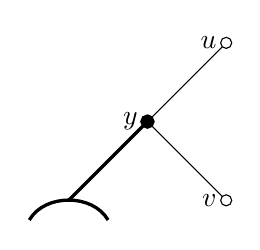
\begin{tikzpicture}[scale=1]
\draw (0,1)--(-1,-0)--(0,-1);
\draw[fill=white] (0,1) circle [radius=2pt]
(0,-1) circle [radius=2pt];
\draw[very thick,fill=black] (-1,0) circle [radius=2pt] (-1,0)--(-2,-1);
\draw[very thick] (-2.5,-1.25) to[out=60,in=120] (-1.5,-1.25);
\node[left] at (0,1) {$u$};
\node[left] at (-1,0) {$y$};
\node[left] at (0,-1) {$v$};
\end{tikzpicture}
\subcaption{$(Y,left)$~left.}
\end{minipage}
\begin{minipage}{0.2\textwidth}
\centering
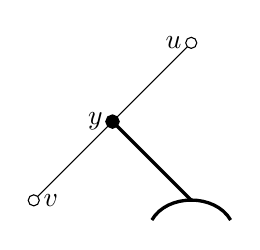
\begin{tikzpicture}[scale=1]
\draw (0,1)--(-2,-1);
\draw[fill=white] (0,1) circle [radius=2pt]
(-2,-1) circle [radius=2pt];
\draw[very thick,fill=black] (-1,0) circle [radius=2pt] (-1,0)--(0,-1);
\draw[very thick] (-0.5,-1.25) to[out=60,in=120] (0.5,-1.25);
\node[left] at (0,1) {$u$};
\node[left] at (-1,0) {$y$};
\node[right] at (-2,-1) {$v$};
\end{tikzpicture}
\subcaption{$(Y,right)$~left.}
\end{minipage}
\begin{minipage}{0.25\textwidth}
\centering
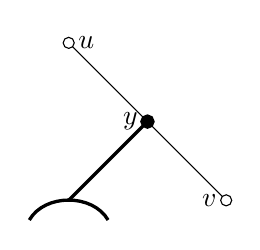
\begin{tikzpicture}[scale=1]
\draw (-2,1)--(0,-1);
\draw[fill=white] (-2,1) circle [radius=2pt]
(0,-1) circle [radius=2pt];
\draw[very thick,fill=black] (-1,0) circle [radius=2pt] (-1,0)--(-2,-1);
\draw[very thick] (-2.5,-1.25) to[out=60,in=120] (-1.5,-1.25);
\node[right] at (-2,1) {$u$};
\node[left] at (-1,0) {$y$};
\node[left] at (0,-1) {$v$};
\end{tikzpicture}
\subcaption{$(Y,left)$~right.}
\end{minipage}
\begin{minipage}{0.2\textwidth}
\centering
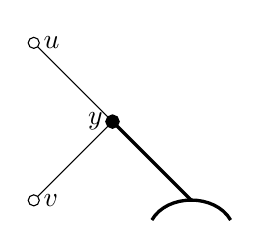
\begin{tikzpicture}[scale=1]
\draw (-2,1)--(-1,0)--(-2,-1);
\draw[fill=white] (-2,1) circle [radius=2pt]
(-2,-1) circle [radius=2pt];
\draw[very thick,fill=black] (-1,0) circle [radius=2pt] (-1,0)--(0,-1);
\draw[very thick] (-0.5,-1.25) to[out=60,in=120] (0.5,-1.25);
\node[right] at (-2,1) {$u$};
\node[left] at (-1,0) {$y$};
\node[right] at (-2,-1) {$v$};
\end{tikzpicture}
\subcaption{$(Y,right)$~right.}
\end{minipage}
\caption{The drawings describe the plug in operation in the different four cases. The bold part highlight the single pair $(Y,S)$.}
\label{fig:plugin}
\end{figure}

Let $(Y,S)$ be a single pair in a rooted subcubic tree $T$, then we {\it remove} $(Y,S)$ from $T$ as follows. Let $y$ be the root of $Y$. If $y$ is the root of $T$, then we obtain an empty tree. If $y$ is a leaf node of $T$, then we obtain $T-y$. Otherwise let $y$ be a non-root and non-leaf node, let $u$ be the parent of $y$ and $v$ be the child of $y$ that is not in $V(Y)$, then we consider the tree obtained from $T$ after replacing $y$ with $v$ as the child of $u$ and deleting $Y$. See Figure~\ref{fig:reduction} for an example.

\begin{figure}[h]
\begin{minipage}{0.5\textwidth}
\centering
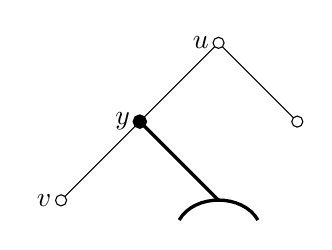
\begin{tikzpicture}[scale=1]
\draw (0,1)--(-2,-1) (0,1)--(1,0);
\draw[fill=white] (0,1) circle [radius=2pt]
(1,0) circle [radius=2pt]
(-2,-1) circle [radius=2pt];
\draw[very thick,fill=black] (-1,0) circle [radius=2pt] (-1,0)--(0,-1);
\draw[very thick] (-0.5,-1.25) to[out=60,in=120] (0.5,-1.25);
\node[left] at (0,1) {$u$};
\node[left] at (-1,0) {$y$};
\node[left] at (-2,-1) {$v$};
\end{tikzpicture}
\end{minipage}
\begin{minipage}{0.1\textwidth}
\centering
\begin{tikzpicture}[scale=1]
\draw (0,1)--(-2,-1) (0,1)--(1,0);
\draw[fill=white] (0,1) circle [radius=2pt]
(1,0) circle [radius=2pt]
(-2,-1) circle [radius=2pt];
\node[left] at (0,1) {$u$};
\node[left] at (-2,-1) {$v$};;
\end{tikzpicture}
\end{minipage}
\caption{The drawing describe an example of the remove operation: a single pair $(Y,right)$ is removed from a subcubic rooted tree. The bold part highlight the single pair $(Y,S)$.}\label{fig:reduction}
\end{figure}

It is clear from the four different plug in cases that if we want to plug in two pairs $(Y,S)$ and $(Y',S')$ on an edge $uv$ such that the ancestor-descendant relationship is given, say $y$ of $Y$ has to be in the path from the root to $y'$ of $Y'$, then we can do these plug ins in any order but with some care. It is the same if we first plug in $(Y,S)$ in the edge $uv$ and then plug in $(Y',S')$ in the edge $yv$ or if we first plug in $(Y',S')$ in the edge $uv$ and then plug in $(Y,S)$ in the edge $uy'$. See Figure~\ref{fig:multiplugin} for the an example.

\begin{figure}[h]
\centering
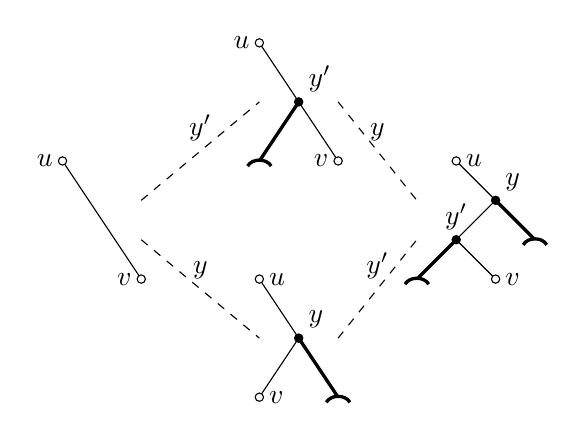
\begin{tikzpicture}[scale=0.5]
\draw[dashed] (-5,0)--(-2,2.5) node[midway,above] {$y'$}
(-5,-1)--(-2,-3.5) node[midway,above] {$y$}
(0,2.5)--(2,0) node[midway,above] {$y$}
(0,-3.5)--(2,-1) node[midway,above] {$y'$};
\draw (-7,1)--(-5,-2) (-2,4)--(0,1) (-2,-2)--(-1,-3.5)--(-2,-5) (3,1)--(4,0)--(3,-1)--(4,-2);
\draw[very thick] (-1,-3.5)--(0,-5) (-1,2.5)--(-2,1) (4,0)--(5,-1) (3,-1)--(2,-2) (-2.3,0.87) to[out=60,in=120] (-1.7,0.87)
(-0.3,-5.13) to[out=60,in=120] (0.3,-5.13) (4.7,-1.13) to[out=60,in=120] (5.3,-1.13) (1.7,-2.13) to[out=60,in=120] (2.3,-2.13);
\draw[fill=white] (-7,1) circle [radius=3pt] (-5,-2) circle [radius=3pt] (-2,4) circle [radius=3pt] (0,1) circle [radius=3pt] (-2,-2) circle [radius=3pt] (-2,-5) circle [radius=3pt] (3,1) circle [radius=3pt] (4,-2) circle [radius=3pt];
\draw[fill=black] (-1,-3.5) circle [radius=3pt] (-1,2.5) circle [radius=3pt] (4,0) circle [radius=3pt] (3,-1) circle [radius=3pt];
\node[left] at (-7,1) {$u$};
\node[left] at (-2,4) {$u$};
\node[right] at (-2,-2) {$u$};
\node[right] at (3,1) {$u$};
\node[left] at (-5,-2) {$v$};
\node[left] at (0,1) {$v$};
\node[right] at (-2,-5) {$v$};
\node[right] at (4,-2) {$v$};
\node[above right] at (4,0) {$y$};
\node[above right] at (-1,-3.5) {$y$};
\node[above right] at (-1,2.5) {$y'$};
\node[above] at (3,-1) {$y'$};
\end{tikzpicture}
\caption{An example of plugging in two pairs $(Y,left)$ and $(Y',right)$ in a left edge $uv$.}
\label{fig:multiplugin}
\end{figure}

For a subset of labels $A\subseteq [k]$, we define the feature template $f_A$ by setting $e(f_A)=1$ if and only if $lab(e)\in A$ and $e(f_A)=0$ otherwise. With a small abuse of notation, we often identify the feature template $f_A$ with the corresponding subset of labels $A$.

\smallskip
Suppose we have a DT such that some feature label~$i$ occurs twice on a path from the root to the leaves, say~$f_1$ is the instance closer to the root and~$f_2$ is the other instance. If~$f_2$ is in the left (resp. right) subtree of~$f_1$, we remove $f_2$'s right (resp. left) subtree. In this case we say we have done an {\it actual removal}.

Suppose we have a feature template labelled~$A$ in our decision tree. Let $A_1,\ldots,A_\ell$ be the sequence of feature templates on the path from the root to~$A$ in order (not including~$A$). Let $A_i'=A_i$ if~$A$ is in the right sub-tree of~$A_i$ and let $A_i'=\overline{A_i}$ otherwise. If $\overline{A} \subseteq A_1' \cup \ldots \cup A_\ell'$, then we remove the subtree rooted at the left child of~$A$. If $A\subseteq \overline{A_1'} \cup \ldots \cup \overline{A_\ell'}$, then we remove the subtree rooted at the right child of~$A$. In this case we say we have done a {\it template removal}. If this procedure has been applied to a record exhaustively, we say that the DT is {\it reduced}.

To be short, for a DT $T$ and a node $v$, we write $v\in T$ instead of $v\in V(T)$ and $v\not\in T$ otherwise. In a DT $T$ we say that path $p$ is a {\it downward} pard path if it is contained in a path having the root as endpoint.

We now formally define two important operations. Given a DT $T$, we say that we {\it reduce} $T$ if we exhaustively do actual removals and template removals. Call $r(T)$ the resulting DT.

Recall that in any DT $T$, every non-leaf node $v$ has one of the following three contents: $v$ is a real feature (without label), or $v$ is a feature with a label, or $v$ is a future feature with the corresponding subset of labels.
A {\it relabelling} $p$ for $T$ is an assignment of contents of $T$ as follows. Every feature is assigned to a feature with is either future, real or with a label. We say that we {\it relabel} the DT $T$ via the relabelling $p$ if for every node of $T$ we apply the corresponding assignment and call $p(T)$ the resulting DT.

The following lemma shows that, after repeatedly applying it the necessary amount of times, to obtain a reduced DT after a sequence of relabels, it is safe to reduce at the end.

\begin{lemma}[Relabelling Lemma]\label{red-last}
Let $T$ be a DT and $p$ be relabelling of $T$. Then $(r \circ p \circ r) (T)=(r \circ p) (T)$.
\end{lemma}

\begin{proof}
For every $v\in T$, we want to prove $v\in (r\circ p\circ r)(T) \Leftrightarrow v\in (r \circ p)(T)$.

$\Rightarrow$ Suppose there is a node $v\not\in (r \circ p)(T)$. Since $v\in p(T)$, there is a set of ancestors of $v$ in $p(T)$ that allows to remove $v$. Let $A_v$ be the union of all the minimal set of ancestors of $v$ in $p(T)$ that allows to remove $v$. If $A_v$ is a set of ancestors of $v$ in $T$ that allows to reduce $v$ then $v\not\in r(T)$ and so $v\not \in (r\circ p\circ r)(T)$. Otherwise let $A'_v$ be the subset of $A_v$ in $(p \circ r)(T)$. We conclude by noting that $A'_v$ contains one of the minimal sets $A_v$ is composed of and so $v\not \in (r\circ p\circ r)(T)$.

$\Leftarrow$ Suppose there is a node $v\not\in (r \circ p \circ r)(T)$. If $v\in (p \circ r)(T)$, there exists a set $A_v$ of ancestors of $v$ in $(p \circ r)(T)$ that allows to reduce $v$. Then $A_v$ is a set of ancestors of $v$ in $p(T)$ that allows to reduce $v$ and so $v\not\in (r \circ p)(T)$. If $v\not\in (p \circ r)(T)$ then $v\not\in r(T)$: there exists a set $A_v$ of ancestors of $v$ in $T$ that allows to remove $v$. This means $A_v$ is a set of ancestors of $v$ in $p(T)$ that allows to remove $v$ and so $v\not\in (r \circ p)(T)$.
\end{proof}

We say that a DT $T$ is a {\it real DT} if every non-leaf node is either a real feature or a future feature, whereas it is a {\it DT template} if it contains no real feature.

Let $B$ be a rooted subcubic tree that corresponds to a $k$-NLC expression of the graph $G_I(E)$.
For $b\in V(B)$, we write $feat(b)$ and $exam(b)$ for the sets of features and examples introduced at nobe $b$.
We say that a real DT $T$ is a DT for the node $b$ if every real feature of $T$ is an element of $feat(b)$ and every example in $exam(b)$ is correctly classified by $T$, i.e. if $e\in exam(b)\cap E^+$ then $e$ ends in a leaf with a $+$ label and if $e\in exam(b)\cap E^-$ then $e$ ends in a leaf with a $-$ label.

Given a real DT $T$ and a node $b\in B$, often we want to perform a very specific composition of operations. Let $p_b$ be the following relabelling of $T$: every real feature of $T$ is assigned to a feature with the label given by the $k$-NLC expression at node $b$ and every other feature is assigned to itself. Then the composition $r \circ p_b$ is called the {\it standard reduction} of $T$ at node $b$.
Given a DT $T$ and a node $b\in B$, it is useful to give the following relabelling $p'_b$: every feature with a label is assigned to the real feature of that node. The relabelling $p'_b$ is called the {\it real relabelling} of $T$ at node $b$.

We say that a DT template $T$ is a DT for the node $b$ if there exits a real DT $T'$ for $b$ such that $T$ is the standard reduction of $T'$. In this case we say that $T'$ is the witness of $T$ for $b$.

\begin{lemma}\label{lem:reduced-tree-height}
If there are $\ell$ features with labels and $2^h$ future features, then every reduced DT template has height at most~$\ell+h$. Furthermore, every path from the root to the leaves contains at most~$\ell$ features with label and at most $h-1$ future features.
\end{lemma}

\begin{proof}
Consider a path~$P$ of maximum length from the root to the leaves in a reduced DT template $T$. 
By the assumptions on $T$, no feature with label appears more than once on this path: the number of these feature nodes on this path is at most~$\ell$. Consider two future features $f_{A}$ and $f_{A'}$ that appear in $P$, say $f_{A}$ is the instance closer to the root. Since $T$ is reduced, we must have that $\emptyset\subset A'\subset A$. Since the label of any future feature has at most $h$ elements, there can be at most $h-1$ feature template nodes on this path. The path ends with a leaf node, so this gives a total of $\ell+h-1+1=\ell+h$ nodes, as required.
\end{proof}

\begin{lemma}\label{lem:reduced-tree-number}
If there are $\ell$ features with label and $2^h$ future features, 
then there are at most $(\ell+2^k+2)2^{\ell+k+1}$ reduced DT templates. Furthermore, these can be enumerated in $\mathcal{O}((\ell+2^k+2)2^{\ell+k+1})$-time.
\end{lemma}

\begin{proof}
By Lemma~\ref{lem:reduced-tree-height}, the tree has height at most $\ell+k$.
Each node of the decision tree could be a feature with label, a future feature, or a leaf: at most $\ell+2^h+2$ different contents. Since there are at most $2^{\ell+h+1}$ nodes in the tree, there are at most $(\ell+2^h+2) 2^{\ell+h+1}$ possible decision trees.
\end{proof}

\smallskip
The {\it semantics} for a record are defined as follows. We say that a pair $(T,s)$ is a {\it record} for the node $b\in B$ and we write $(T,s)\in \mathcal{R}(b)$, if $T$ is a DT template for $b$ and $s$ is the minimum number of elements that have been deleted from a witness $T'$ of $T$ for $b$.

\subsection{Proof to the Main Result}

Now, it suffices to compute $\mathcal{R}(b)$ via leaf-to-root dynamic programming. The following four lemmas show how this can be achieved for all of the four types of nodes in a $k$-NLC expression tree $B$.

\begin{lemma}[leaf node]\label{lem:leaf}
Let $b\in V(B)$ be a leaf node. Then $\mathcal{R}(b)$ can be computed in time $\mathcal{O}(k(2^k+3)2^{k+2})$.
\end{lemma}

\begin{proof}
Let $v$ be the vertex of $G_I(E)$ that corresponds to the leaf node $b$. This means either $v\in E$ or $v\in feat(E)$.

We have to enumerate all possible reduced DT templates $T$ for $b$. It is enough to consider all reduced DT templates $T$ of height at most $k+1$ and discard those that are not DT templates for $b$; these can be enumerated in time $\mathcal{O}((2^k+3)2^{k+2})$ by Lemma~\ref{lem:reduced-tree-number} and the check can be done in time $\mathcal{O}(k)$. We add the pair $(T,0)$ to the set of records $\mathcal{R}(b)$. 

Now we have to show the correctness of the construction for $\mathcal{R}(b)$, i.e. $(T,s)\in \mathcal{R}(b)$ if and only if $s$ is the minimum number of elements that have been deleted from a witness $T'$ of $T$ for $b$.

We start with the forward direction. Let $(T,s)\in \mathcal{R}(b)$. By construction, we have that $s=0$ and $T$ is a DT template for $b$ which is already reduced. Then $T$ is trivially a witness of $T$ for $b$.

Now we prove the backward direction. Let $T$ be a reduced DT template such that $0$ is the minimum number of elements that have been deleted from a witness $T'$ of $T$ for $b$. This means $T'$ is obtained from $T$ after the real relabelling at node $b$ is applied: $T$ is a DT template among the considered DTs above which leads to the fact that $(T,0)\in \mathcal{R}(b)$.
\end{proof}

\begin{lemma}[join node]\label{lem:join}
Let $b\in V(B)$ be a join node. Then $\mathcal{R}(b)$ can be computed in time $\mathcal{O}()$.
\end{lemma}

\begin{proof}
Let $b_L$ and $b_R$ be the left, resp. right, child of $b$ in $B$: we may assume the labels for $feat(b_L)$ are in $[k]$ and the labels for $feat(b_R)$ are in $[k']$. Moreover, let $M$ be the $k\times k$ $\{0,1\}$ matrix that represent the node $b$. Finally, for every label $i\in [k]$, let $A_i=\{j\in [k]~|~M_{i,j}=1\}$.

We consider every reduced DT $T$ for $b$ with feature labels in $[k]\cup [k']$ and future feature labels in $\mathcal{P}([k])$; these can be enumerated in time $\mathcal{O}((2k+2^k+2)2^{3k+1})$ by Lemma~\ref{lem:reduced-tree-number}.

For every such DT $T$, we create a DT $T_L$ as follows. Let $p_*$ be the following relabelling: for every $i'\in [k']$, every feature with label $i'$ is assigned to the future feature $A_i$. Then we apply the composition $r \circ p_*$ to $T$. In a symmetrical way we create a DT $T_R$. Let $p'_*$ be the following relabelling: for every $i\in [k]$, every feature with label $i$ is assigned to the future feature $A_{i'}$ and every future feature $A_i$ is assigned to the future feature $A_{i'}$. Then we apply the composition $r \circ p'_*$ to $T$.

Now we want to understand if there is a record in $\mathcal{R}(b_L)$ of the form $(T_L,s_L)$ for some positive integer $s_L$ and if there is a record in $\mathcal{R}(b_R)$ of the form $(T_R,s_R)$ for some positive integer $s_R$: if the answer is yes in both cases, we add a record $(T,s_L+s_R)$ to $\mathcal{R}(b)$; otherwise we discard this option.

\medskip
Now we want to evaluate the running time of computing $\mathcal{R}(b)$. Every reduced DT $T$ can be enumerated in time $\mathcal{O}((2k+2^k+2)2^{3k+1})$ by Lemma~\ref{lem:reduced-tree-number}.
For every such tree $T$, there are at most $2^{3k}$ paths from the root to the leaves and for every of these paths there are at most $k$ nodes for each of the following features: with label in $[k]$, with label in $[k']$ and future by Lemma~\ref{lem:reduced-tree-height}.
This means $p_*$ and $p'_*$ can be done in $\mathcal{O}(k2^{3k})$ time.
%GP: to understand the complexity for $r$.

\medskip
Now we have to show the correctness of the construction for $\mathcal{R}(b)$. We start with the forward direction. Let $(T,s)\in \mathcal{R}(b)$. By construction there exist records $(T_L,s_L)\in \mathcal{R}(b_L)$ and $(T_R,s_R)\in \mathcal{R}(b_R)$ such that $T_L$ and $T_R$ are obtained by the application of $r \circ p_*$ and $r \circ p'_*$ respectively to $T$ and $s_L+s_R=s$.

By induction, for $H\in \{L,R\}$, we know that $s_H$ is the minimum number of elements that have been deleted from a witness $T'_H$ of $T_H$ for $b_H$.

For $H\in \{L,R\}$, we define maps $x_H$ and $y_H$ as follows. Let $x_H~:~V(T_H)\to V(T)$ and $y_H~:~V(T_H)\to V(T'_L)$ be the functions that maps every node of $T_H$ to the corresponding node in $T$ and in $T'_L$ and note that by constructions both these maps are injective. 

\begin{figure}[h]
\centering
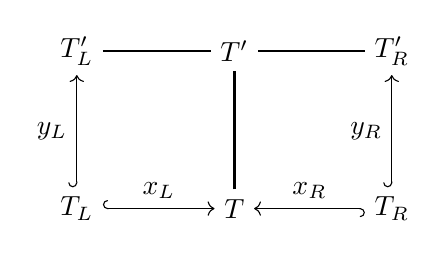
\begin{tikzpicture}
\node (1) at (-2,1) {$T'_L$};
\node (2) at (0,1) {$T'$};
\node (3) at (2,1) {$T'_R$};
\node (4) at (-2,-1) {$T_L$};
\node (5) at (0,-1) {$T$};
\node (6) at (2,-1) {$T_R$};
\draw[right hook->] (4)--(5) node[midway,above] {$x_L$};
\draw[right hook->] (6)--(5) node[midway,above] {$x_R$};
\draw[right hook->] (4)--(1) node[midway,left] {$y_L$};
\draw[right hook->] (6)--(3) node[midway,left] {$y_R$};
\draw[thick] (1)--(2);
\draw[thick] (3)--(2);
\draw[very thick] (5)--(2);
\end{tikzpicture}
\end{figure}

Moreover, $V(T)\setminus Im(x_H)$ and $V(T'_H)\setminus Im(y_H)$ can be partitioned into subtrees that have been deleted after the application of $r\circ p_*$, $r\circ p'_*$ on $T$ or of the standard reduction on $T'_H$: let $X^*_H$ and $Y^*_H$ be the set of roots of the above subtrees in $V(T)\setminus Im(x_H)$ and $V(T'_H)\setminus Im(y_H)$ respectively.  
In addition, for every element $y\in Y^*_H$, let $Y^H_y$ be the maximal subtree of $T'_H$ rooted at $y$ with no elements from $Im(y_H)$ and that does not contain any vertex from $Y^*_H\setminus \{y\}$; let $(Y^H_y,S^H_y)$ the corresponding single pair.
%GP: add figure
In a similar way, for every element $x\in X^*_H$, let $X^H_x$ be the maximal subtree of $T$ rooted at $x$ with no elements from $Im(x_H)$ and that does not contain any vertex from $X^*_H\setminus \{x\}$; let $(X^H_x,S^H_x)$ the corresponding single pair. 
Finally, for every $y\in Y^*_H$, let $P^H_y$ be the shortest downwards path in $T'_H$ that contains $y$ and with both endpoints in $Im(y_H)$, say $y_H(t)$ and $y_H(t')$. 

\smallskip
\noindent
{\it Claim 1: For every $H\in \{L,R\}$ and for every $y,y'\in Y^*_H$, the paths $P^H_{y}$ and $P^H_{y'}$ are either edge disjoint or $P^H_{y}=P^H_{y'}$.}

\noindent
{\it Proof.} If $P^H_{y}$ and $P^H_{y'}$ are edge disjoint, then the statement is proven immediately. Suppose $P^H_{y}$ and $P^H_{y'}$ share an edge. By minimality and the fact they are downwards paths, $P^H_{y}$ and $P^H_{y'}$ share the endpoint towards the root. If they also share the other endpoint, then the statement is proven immediately. Suppose now their endpoints towards the leaves is different, say $w$ and $w'$, and consider the last edge those paths have in common in a root-to-leaf order, say $uv$. 

Without loss of generality, we can assume $w$ belongs to the left branch of $v$ and $w'$ belongs to the right branch of $v$. Note that $v\in V(T'_H)\setminus Im(y_H)$, or we get a contradiction due the minimality of $P^H_y$.
Now we get the following contradiction: by construction, $w$ and $w'$ are both elements of $Im(y_H)$ but at least one of them must be in $V(T'_H)\setminus Im(y_H)$ since it is an element of either $Y^H_{y}$ or of $Y^H_{y'}$. This proves Claim 1.

\smallskip
Now for every $y\in Y^*_H$ we consider the path $Q^H_y$ in $T$ having endpoints $x_H(t)$ and $x_H(t)$.

\smallskip
Now we are able to describe how to obtain a witness $T'$ of $T$ for $b$. 
For every $y\in Y^*_L$, in the last edge of path $Q^L_y$ we plug in the single pair $(Y^L_{y'},S^L_{y'})$ rooted at $y'$, for every internal node $y'$ of $P^L_y$, in the order the nodes $y'$ apprear in $P^L_y$. Note that, in the case an element of $Y^*_L$ is present in more than one $P^L_y$, we plug in the corresponding single pair only once. Note also that whenever we plug in some single pair $(Y^L_{y},S^L_{y})$ in a DT, the tree $Y^L_{y}$ has real features and future features as nodes. Call this graph $T^*$. Now we do the same sequence of plug ins of the single pairs corresponding to the internal vertices of $P^R_y$ in the last edge of the path $Q^R_y$. Again, in the case an element of $Y^*_R$ is present in more than one $P^R_y$, we plug in the corresponding single pair only once. Call the tree obtained in this way $T'$. Node that $T'$ contains real features from $feat(b_L)$ and from $feat(b_R)$ and future features with labels in $\mathcal{P}([k])$.

\smallskip
To conclude this part of the proof we have to show two things: $(i)$ $T$ is obtained from $T'$ after removing $s$ vertices; $(ii)$ $T'$ is a real DT for $b$. We start proving $(i)$: by construction $T'$ is obtained from $T$ after adding $s_L$ elements from $T'_L$ and $s_R$ elements from $T'_R$, and so with $s_L+s_R=s$ more elements. 

Before considering statement $(ii)$, we consider the following relabelling $p_+$ of $T'$: every real feature in $feat(b_R)$ is a assigned to a feature with its label at node $b_R$ and every other feature is assigned to itself. The real DT $T'_L$ can be obtained from $T'$ by the application of the composition $r \circ p_* \circ p_+$.

Now we consider statement $(ii)$. We show that given an example $e\in exam(b_L)$, $e$ is correctly classified by $T'$ and to do so we show that $e$ ends in a leaf of $T'$ that corresponds to the leaf where $e$ ends in $T'_L$. 
Say that $e$ goes along a path $P$ of $T'_L$ from the root to a leaf $\ell$ and let $Q$ be the corresponding path in $T'$, i.e. the path from $r$ to $\ell$ (note that by construction $\ell$ is present in $T'$ and is still a leaf). 
Let $v$ be a node of $Q$, we can have the following different cases.

\begin{itemize}
\item $v$ is a real feature from $feat(b_L)$: $v$ is also present in $T'_L$ as real feature; 
\item $v$ is a real feature from $feat(b_R)$: $v$ might not be present in $T'_L$ due reductions but if it is present it is a future feature $A_i$ for some $i\in [k]$;
\item $v$ is a future feature $f_A$: $v$ might not be present in $T'_L$ due reductions but if it is present it is still the same future feature $A_i$.
\end{itemize}

If $v$ is present in $T'_L$ then the behaviour of $v$ on $e$ in $T'_L$ and in $T'$ is the same. Suppose now $v$ is a node of $Q$ that is being reduced due his label and so it is not present in $T'_L$. This means there is a set of ancestors of $v$ such that their labels allows to remove $v$ and by construction $v$ behaves on $e$ like those ancestors. This proves $e$ goes along $Q$ and in particular it ends at leaf $\ell$ and so $T'$ is a real DT for $b_L$. With symmetric construction, we show that $T'$ is also a real DT for $b_R$.

\medskip
Now we prove the backward direction. Let $T$ be a reduced DT such that $s$ is the minimum number of elements that have been deleted from a witness $T'$ of $T$ for $b$. In particular, we recall that $T'$ is a real DT for $b$ with actual feature labels in $[k]\cup [k']$ and future feature labels in $\mathcal{P}([k])$. 

We create at real DT $T'_L$ by the application of the composition $r \circ p_* \circ p_+$ to $T'$. By assumption $T'$ is a real DT for $b_L$ and by construction $T'_L$ is a real DT for $b_L$. 
Denote with $T_L$ the DT template obtained from $T'_L$ by standard reduction and denote with $s_L$ the number of nodes that have been deleted from $T'_L$ to obtain $T$. By induction we have $(T_L,s_L)\in \mathcal{R}(b_L)$.
Now we note that $T_L$ is obtained from $T$ after the application of the composition $r \circ p_*$. In a symmetric way, we construct $T'_R$, $T_R$ and the record $(T_R,s_R)\in \mathcal{R}(b_R)$. Then $(T,s_L+s_R)\in \mathcal{R}(b)$.
\end{proof}

\begin{lemma}[relabel node]\label{lem:relabel}
Let $b\in V(B)$ be relabel node. Then $\mathcal{R}(b)$ can be computed in time $\mathcal{O}()$.
\end{lemma}

\begin{proof}
Let $b_C$ be the unique child of $b$ in $B$. Let $R$ be the mapping of $[k]$ to itself that represent the node $b$. Moreover, since we are considering a {\it nice} NLC-expression we can assume $R$ is the identity mapping, i.e. $R(\ell)=\ell$, for all values except for a unique element $i$ of its domain, i.e. $R(i)=j$ for some $j\in [k]\setminus \{i\}$.

We say that a future feature $A$ is {\it good} if it does not distinguish between $i$ and $j$, that is $i\in A$ if and only if $j\in A$, and {\it bad} otherwise. Let $(T_C,s_C)$ be an element of $\mathcal{R}(b_C)$. Let $p''$ the following relabelling of the DT template $T_C$: every feature with label $i$ is assigned to label $j$ and every future feature with label $A$ is assigned to the future feature with label $A\setminus \{i\}$. 

If $T_C$ has a bad future feature then we do not take any other action. Suppose now $T_C$ has only good future features; now let $T$ be the DT template obtained from $T_C$ after the application of the composition $r \circ p''$ and let $s^*$ be the number of nodes that have been deleted from $T_C$ to $T$.

If there is a record in $\mathcal{R}(b)$ of the form $(T,s')$ for some integer $s'\leq s_C+s^*$ then we do not take any other action.
If there is a record in $\mathcal{R}(b)$ of the form $(T,s')$ for some integer $s'>s_C+s^*$ then we replace it with $(T,s_C+s^*)$.
If there is no record in $\mathcal{R}(b)$ of the form $(T,s')$ for some integer $s'$ then we add $(T,s_C+s^*)$ to $\mathcal{R}(b)$.

\medskip
Now we have to show the correctness of the construction for $\mathcal{R}(b)$, i.e. $(T,s)\in \mathcal{R}(b)$ if and only if $s$ is the minimum number of elements that have been deleted from a witness $T'$ of $T$ for $b$.

\smallskip
We start with the forward direction. Let $(T,s)\in \mathcal{R}(b)$. By construction there exists a record $(T_C,s_C)\in \mathcal{R}(b_C)$ such that $T$ is obtained from $T_C$ after the application of $r \circ p''$ and let $s^*=s-s_C$. By induction $s_C$ is the minimum amount of nodes that have been deleted from a witness $T'_C$ of $T_C$ for $b_C$. By construction we also know that every future feature of both $T'_C$ and $T_C$ is good.

Denote with $T'$ the real DT obtained $T'_C$ after the application of $r \circ p''$: note that this last reduction does not any node since every future feature of $T'_C$ is good and there is no feature with label $i$. To conclude this part of the proof we have to show two things: $(i)$ $T$ is obtained from $T'$ after removing $s$ vertices; $(ii)$ $T'$ is a witness of $T$ for $b$. 

Before proving $(i)$, we describe how $T$ can be obtained from $T'$. Let $p'''$ be the following relabelling of $T'$: every real feature that contains $j$ is assigned to the real feature $A\cup \{i\}$ and every other feature is assigned to itself. Then the application of the composition $p'''$, the standard reduction and $r \circ p''$ to $T'$ is exactly the standard reduction for $T'$ which then result to the DT template $T$.
By Lemma~\ref{red-last} the score of the standard reduction from $T'$ to $T$ is exactly $s_C+s^*=s$. 

Now we consider statement $(ii)$. First note that $exam(b)=exam(b_C)$.
We show that a given example $e\in exam(b)$ is correctly classified by $T'$. Say that $e$ goes along a path $P$ of $T'_C$ from the root to a leaf $\ell$. We show $e$ goes along the path $P$ in $T'$ as well: every real feature has not changed and so $e$ behaves the same. Since every future feature of $T'_C$ is good, then $e$ behave the same on the corresponding future feature of $T'$.

\smallskip
Now we prove the backward direction. Let $T$ be a reduced DT such that $s$ is the minimum number of elements that have been deleted from a witness $T'$ of $B$ for $b$. In particular, we recall that real $T'$ is a DT for $b$ with real features and future feature labels in $\mathcal{P}([k]\setminus \{i\})$.

We create the real DT $T'_C$ as the application of $r \circ p'''$ to $T'$, the DT template $T_C$ as the application of the standard reduction to $T'_C$. By construction we have $(T_C,s_C)\in \mathcal{R}(b_C)$, where $s_C$ is the number of nodes that have been removed from $T'_C$ to $T_C$. Note that $T_C$ has only good future features.
Finally we note that $T$ is obtained from $T_C$ by the application of $r \circ p''$.
\end{proof}

Now we can finally prove Theorem~\ref{the:trac-nlcw-b-td} and Theorem~\ref{the:trac-tw-b}, which we restate here.

\smallskip
\noindent
{\bf Theorem~\ref{the:trac-nlcw-b-td} (restated).}
{\it Let $E$ be a CI, let $(B,\chi)$ be an NLC-expression decomposition of width $k$ for $G_I(E)$, and let $s$ be an integer. Then, deciding whether $E$ has a DT of size at most $s$ is fixed-parameter tractable parameterized by $k$. In particular, such computation takes $\mathcal{O}()$ time.}

\begin{proof}
We start off by computing $\mathcal{R}(b)$ for every node $b$ of $B$, via leaf-to-root dynamic programming. An upper bound for the running time for this step is the number of nodes of $B$ times the maximum running time to compute the record at each node which is given by Lemmas~\ref{lem:leaf}, \ref{lem:join} and \ref{lem:relabel}.

Now we look at the root node $r$ of $B$. We go through all the records of $\mathcal{R}(r)$ and select a record $(T,s)\in \mathcal{R}(r)$ such that $|T|+s$ is minimum over all DTs with no future feature.
\end{proof}

\smallskip
\noindent
{\bf Theorem~\ref{the:trac-tw-b} (restated).}
{\it \DTL{} is fixed-parameter tractable parameterized by NLC-width.}





\section{Conclusion}
We have initiated the study of the parameterized complexity of learning DTs from data. Our main tractability result provides novel insights into the structure of DTs and is based on the NLC-width parameter that seems to be well suited to measure the complexity of input instances for the problem.

The problem of learning DTs comes in many variants and flavors, which opens up a wide range of new research directions to explore. For instance:

\begin{itemize}
\item What other (structural) parameters can be exploited to efficiently learn DTs? Is learning DTs of small size fixed-parameter tractable parameterized by the rank-width of $G_I(E)$?
\item Instead of learning DTs of small size, one often wants to learn DTs of small height. Therefore, it is natural to ask whether our approach can be also used in this setting. While one can adapt our approach to obtain an XP-algorithm for learning DTs of small height parameterized by NLC-width, it is not clear to us whether the problem also allows for an fpt-algorithm. 
\item Can we extend our approach to CIs, where features range over an arbitrary domain? In this case, one usually still uses DTs that make binary decisions (i.e. whether a feature is smaller equal or larger than a given threshold). While it is relatively easy to see that our approach can be extended if the  domain's size (for every feature) is bounded or used as an additional parameter, it is not clear what happens if the size of the domain is allowed to grow arbitrarily.
\end{itemize}

\bibliography{literature}
\end{document}